%-----------------------------------------------------------------------------%
\addChapter{Lampiran 1}
\chapter*{Lampiran 1: Contoh file input}
\label{lamp:inputExample}
%-----------------------------------------------------------------------------%
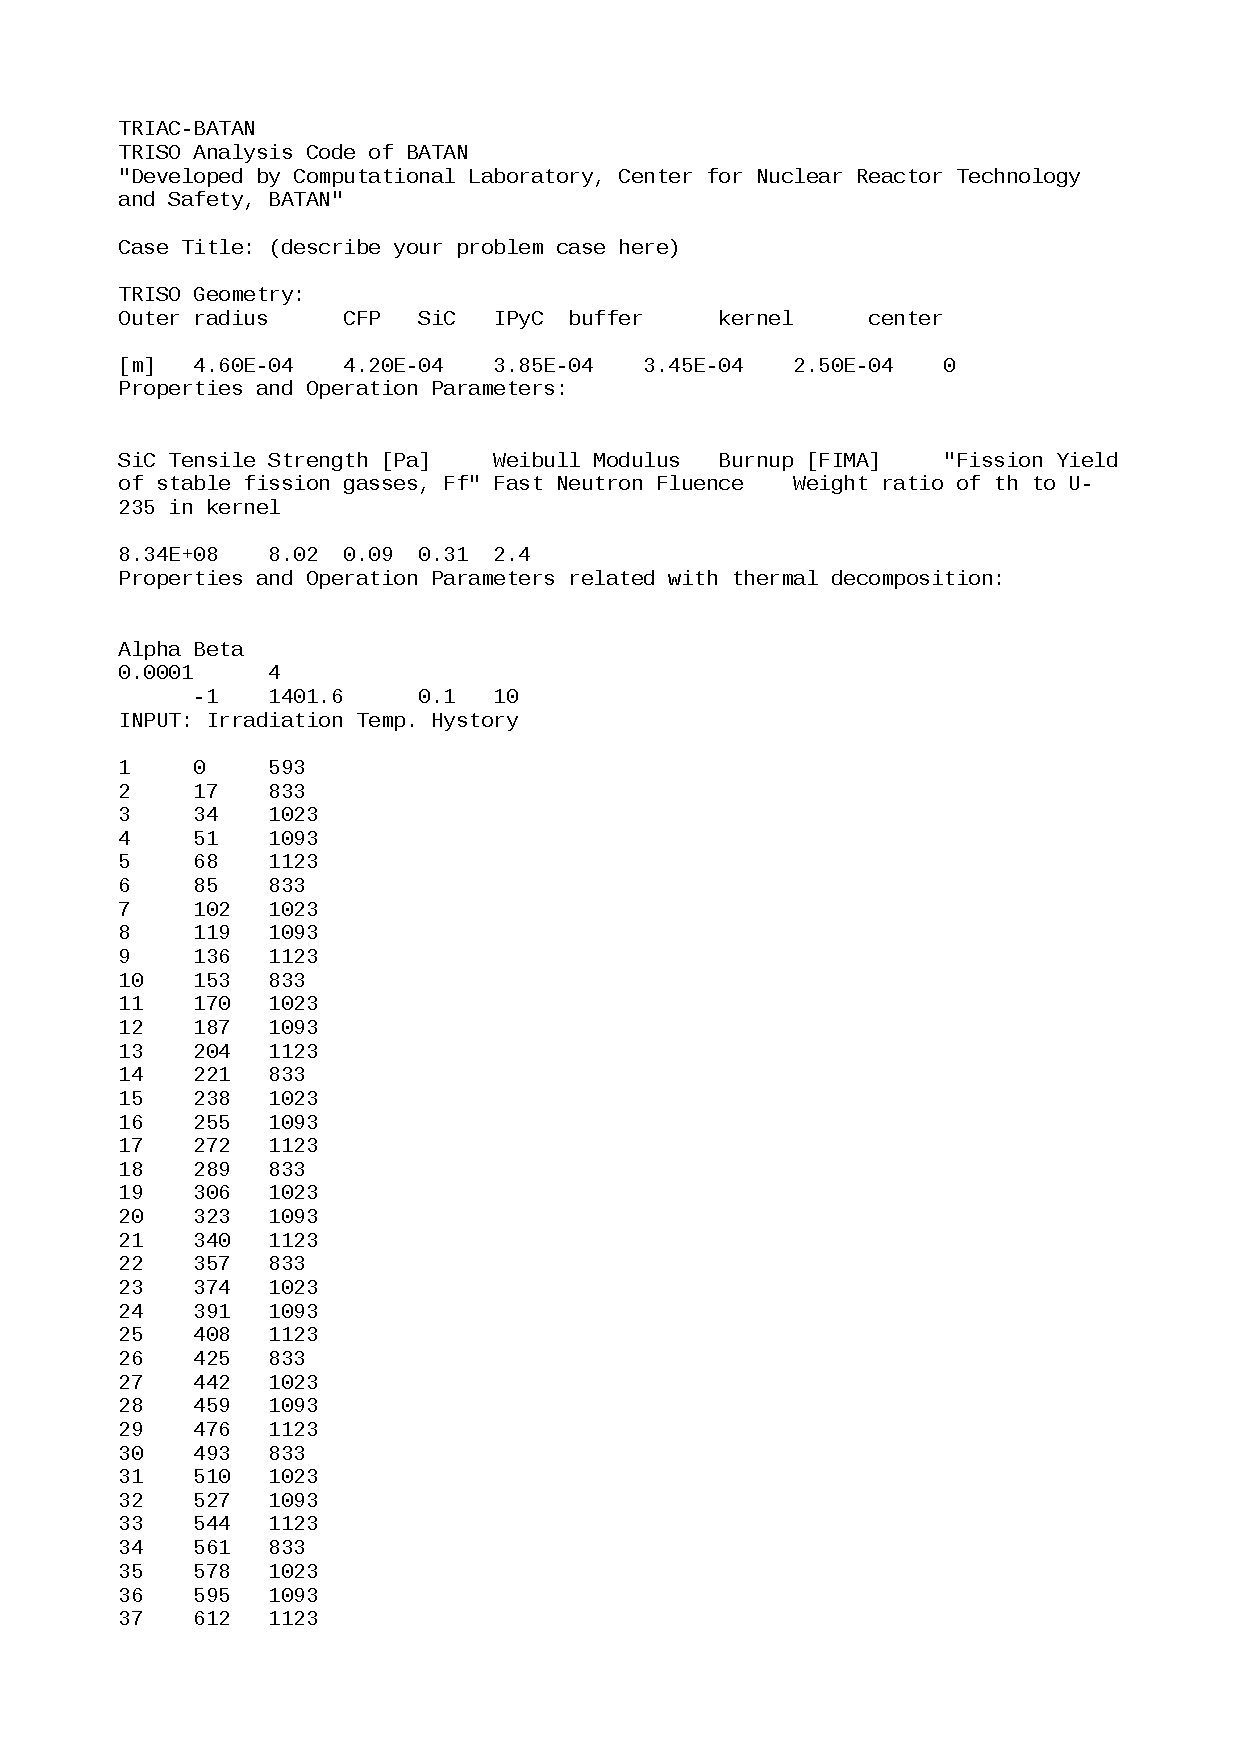
\includepdf[pages={1-}]{inputExample.pdf}
%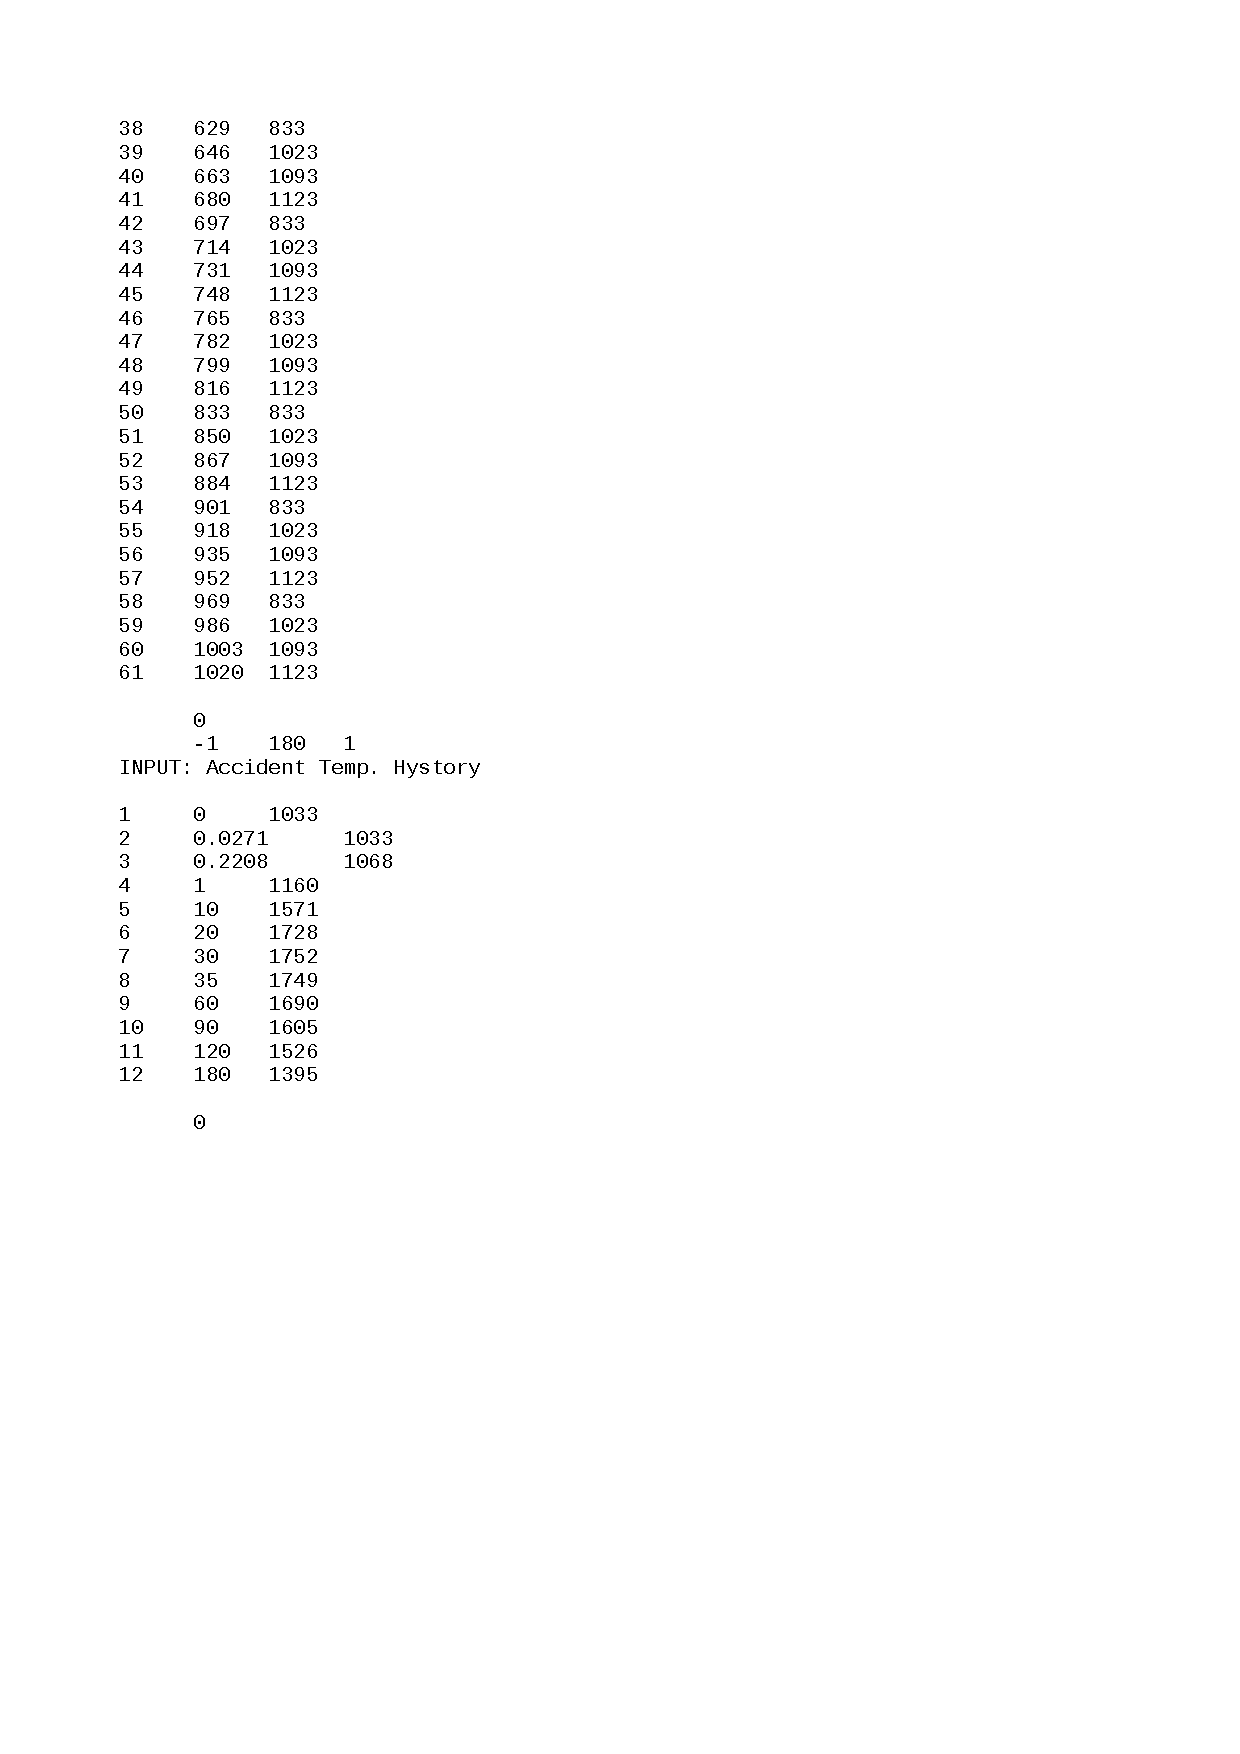
\includepdf{inputExample2}

\addChapter{Lampiran 2: InputData.py}
\chapter*{Lampiran 2: InputData.py}
\scriptsize
\lstinputlisting[language=python, numbers=left, numberstyle=\tiny, caption=InputData.py, showstringspaces=false, label=InputData.py]{../Uji/InputData.py}
\normalsize

\addChapter{Lampiran 3: interpolasi.py}
\chapter*{Lampiran 3: interpolasi.py}
\scriptsize
\lstinputlisting[language=python, numbers=left, numberstyle=\tiny, caption=Interpolasi.py, showstringspaces=false, label=Interpolasi.py]{../TRIAC/Interpolasi.py}
\normalsize

\addChapter{Lampiran 4: core.py}
\chapter*{Lampiran 4: core.py}
\scriptsize
\lstinputlisting[language=python, numbers=left, numberstyle=\tiny, caption=core.py, showstringspaces=false, label=core.py]{../Uji/core.py}
\normalsize

\addChapter{Lampiran 5: triac.py}
\chapter*{Lampiran 5: triac.py}
\scriptsize
\lstinputlisting[language=python, numbers=left, numberstyle=\tiny, caption=triac.py, showstringspaces=false, label=triac.py]{../Uji/triacc.py}
\normalsize
